\documentclass[10pt]{article}
\usepackage[letterpaper]{geometry}
\geometry{verbose,tmargin=1in,bmargin=1in,lmargin=1in,rmargin=1in}
\usepackage{setspace}
\usepackage{ragged2e}
\usepackage{color}
\usepackage{titlesec}
\usepackage{graphicx}
\usepackage{float}
\usepackage{mathtools}
\usepackage{amsmath}
\usepackage[font=small,labelfont=bf,labelsep=period]{caption}
\usepackage[english]{babel}
\usepackage{indentfirst}
\usepackage{array}
\usepackage{makecell}
\usepackage[usenames,dvipsnames]{xcolor}
\usepackage{multirow}
\usepackage{tabularx}
\usepackage{arydshln}
\usepackage{caption}
\usepackage{subcaption}
\usepackage{xfrac}
\usepackage{etoolbox}
\usepackage{cite}
\usepackage{url}
\usepackage{dcolumn}
\usepackage{hyperref}
\usepackage{courier}
\usepackage{url}
\usepackage{esvect}
\usepackage{commath}
\usepackage{verbatim} % for block comments
\usepackage{enumitem}
\usepackage{hyperref} % for clickable table of contents
\usepackage{braket}
\usepackage{titlesec}
\usepackage{booktabs}
\usepackage{gensymb}
\usepackage{longtable}
\usepackage{listings}
\usepackage{cancel}
\usepackage{amsmath}
\lstset{
    frame=single,
    breaklines=true,
    postbreak=\raisebox{0ex}[0ex][0ex]{\ensuremath{\color{red}\hookrightarrow\space}}
}

% for circled numbers
\usepackage{tikz}
\newcommand*\circled[1]{\tikz[baseline=(char.base)]{
            \node[shape=circle,draw,inner sep=2pt] (char) {#1};}}


\titleclass{\subsubsubsection}{straight}[\subsection]

% define new command for triple sub sections
\newcounter{subsubsubsection}[subsubsection]
\renewcommand\thesubsubsubsection{\thesubsubsection.\arabic{subsubsubsection}}
\renewcommand\theparagraph{\thesubsubsubsection.\arabic{paragraph}} % optional; useful if paragraphs are to be numbered

\titleformat{\subsubsubsection}
  {\normalfont\normalsize\bfseries}{\thesubsubsubsection}{1em}{}
\titlespacing*{\subsubsubsection}
{0pt}{3.25ex plus 1ex minus .2ex}{1.5ex plus .2ex}

\makeatletter
\renewcommand\paragraph{\@startsection{paragraph}{5}{\z@}%
  {3.25ex \@plus1ex \@minus.2ex}%
  {-1em}%
  {\normalfont\normalsize\bfseries}}
\renewcommand\subparagraph{\@startsection{subparagraph}{6}{\parindent}%
  {3.25ex \@plus1ex \@minus .2ex}%
  {-1em}%
  {\normalfont\normalsize\bfseries}}
\def\toclevel@subsubsubsection{4}
\def\toclevel@paragraph{5}
\def\toclevel@paragraph{6}
\def\l@subsubsubsection{\@dottedtocline{4}{7em}{4em}}
\def\l@paragraph{\@dottedtocline{5}{10em}{5em}}
\def\l@subparagraph{\@dottedtocline{6}{14em}{6em}}
\makeatother

\newcommand{\volume}{\mathop{\ooalign{\hfil$V$\hfil\cr\kern0.08em--\hfil\cr}}\nolimits}

\setcounter{secnumdepth}{4}
\setcounter{tocdepth}{4}
\begin{document}

\title{ME 280a: HW 3}
\author{April Novak}

\maketitle

\section{Introduction and Objectives}

The purpose of this study is to solve a simple finite element (FE) problem using a Preconditioned Conjugate-Gradient (PCG) solver, with a diagonal preconditioner. This involves the storage of the information element-by-element. So, while the problem to be solved is similar to past assignments, the numerical solution method is modified. In addition, the elastic modulus is allowed to be a function of position. The Galerkin FE method is used, which for certain classes of problems possesses the ``best approximation property,'' a characteristic that signifies that the FE solution obtained is the best possible solution for a given mesh refinement and choice of shape functions. The mathematical procedure and numerical implementation is described in Section \ref{sec:Procedure}.

\section{Procedure}
\label{sec:Procedure}

This section details the problem statement and mathematical method used for solving the problem.

\subsection{Problem Statement}

This section describes the mathematical process used to solve the following problem:

\begin{equation}
\label{eq:Problem}
\begin{aligned}
\frac{d}{dx}\left(E(x)\frac{du}{dx}\right)=xk^3\cos{\left(\frac{2\pi kx}{L}\right)}\\
\end{aligned}
\end{equation}

where \(E\) is the modulus of elasticity, \(u\) is the solution, \(k\) is a known constant, \(L\) is the problem domain length, and \(x\) is the spatial variable. For simplicity, a constant \(\gamma=2\pi k/L\) is defined. In order to verify that the program functions correctly, the FE solution to Eq. \eqref{eq:Problem} will be compared with the analytical solution to Eq. \eqref{eq:Problem}. To determine the analytical solution, integrate Eq. \eqref{eq:Problem} once to obtain:

\begin{equation}
\label{eq:Problem2}
E(x)\frac{du}{dx}=k^3\left\lbrack \frac{x}{\gamma}\sin{(\gamma x)}+\frac{1}{\gamma^2}\cos{(\gamma x)}\right\rbrack+C_1
\end{equation}

where, even though \(E\) is a function of \(x\), it is constant over particular lengths of the domain. Hence, the analytical solution can be determined by splitting up the domain into sufficiently small regions where \(E\) is constant. So, for the remainder of this section, \(E\) is treated as constant, and it is understood that the analytical solutions obtained are exact only over each individual region where \(E\) is constant. Integrating once more:

\begin{equation}
\label{eq:Problem3}
u(x)=\frac{1}{E(x)}\left\lbrack\frac{-xk^3}{\gamma^2}\cos{(\gamma x)}+\frac{2k^3}{\gamma^3}\sin{(\gamma x)}\right\rbrack+\frac{C_1x}{E(x)}+C_2
\end{equation}

The boundary conditions for this problem are Dirichlet at both endpoints, such that:

\begin{equation}
\begin{aligned}
u(0)=-0.1\\
u(L)=0.7\\
\end{aligned}
\end{equation}

From Eq. \eqref{eq:Problem}, \(E(x)du/dx\) must be continuous in the domain, and must match at inter-block boundaries. For example, for two blocks that share a node at \(x=x_{share}\):

\begin{equation}
\begin{aligned}
k^3\left\lbrack \frac{x_{share}}{\gamma}\sin{(\gamma x_{share})}+\frac{1}{\gamma^2}\cos{(\gamma x_{share})}\right\rbrack+C_1(\text{block 1})=\quad\\
k^3\left\lbrack \frac{x_{share}}{\gamma}\sin{(\gamma x_{share})}+\frac{1}{\gamma^2}\cos{(\gamma x_{share})}\right\rbrack+C_1(\text{block 2a})\\
\end{aligned}
\end{equation}

Because all constants besides \(E\) are constant in the domain, \(C_1\) is the same for each block. The second requirement is that \(u\) be continuous across block edges. From Eq. \eqref{eq:Problem3}:

\begin{equation}
\begin{aligned}
\frac{1}{E(\text{block 1})}\underbrace{\left\lbrack\frac{-x_{share}k^3}{\gamma^2}\cos{(\gamma x_{share})}+\frac{2k^3}{\gamma^3}\sin{(\gamma x_{share})}\right\rbrack}_\text{\circled{A}}+\frac{C_1(\text{block 1})x_{share}}{E(\text{block 1})}+C_2(\text{block 1})=\quad\\
\frac{1}{E(\text{block 2})}\left\lbrack\frac{-x_{share}k^3}{\gamma^2}\cos{(\gamma x_{share})}+\frac{2k^3}{\gamma^3}\sin{(\gamma x_{share})}\right\rbrack+\frac{C_1(\text{block 2})x_{share}}{E(\text{block 2})}+C_2(\text{block 2})\\
\end{aligned}
\end{equation}

Rearranging, and recognizing that \(C_1\) is the same for all blocks, the following must be true at each shared location:

\begin{equation}
\begin{aligned}
\label{eq:Shared}
C_1\left(\frac{x_{share}}{E(\text{left})}-\frac{x_{share}}{E(\text{right})}\right)+C_2(\text{left})-C_2(\text{right})=-\circled{A}\left(\frac{1}{E(\text{left})}-\frac{1}{E(\text{right})}\right)
\end{aligned}
\end{equation}

Then, at the left endpoint:

\begin{equation}
\label{eq:Left}
C_2(\text{block 1})=u(0)
\end{equation}

And at the right endpoint:

\begin{equation}
\label{eq:Right}
\frac{C_1(\text{last block})L}{E(L)}+C_2(\text{last block})=u(L)-\frac{1}{E(x)}\left\lbrack\frac{-Lk^3}{\gamma^2}\cos{(\gamma L)}+\frac{2k^3}{\gamma^3}\sin{(\gamma L)}\right\rbrack
\end{equation}

Eq. \eqref{eq:Left} and Eq. \eqref{eq:Right} provide two boundary conditions, while Eq. \eqref{eq:Shared} provides one boundary condition at each shared location (locations at which \(E\) changes). This, combined with the fact that \(C_1\) is the same for each element, provides a system of linear equations that can be solved to obtain \(C_1\) and \(C_2(\text{block 1}, \text{block 2}, \text{block 3}, \text{block 4}, \cdots, \text{block 10})\). This is the method used in this assignment to determine the analytical solution. The method is made very general so that any number of piecewise-constant regions of \(E\) can be solved both analytically and with the FEM. The analytical solution is plotted below, and the values for the coefficients \(C_1\) and \(C_2\) in each block are given in the following table.

\begin{figure}[H]
\begin{center}  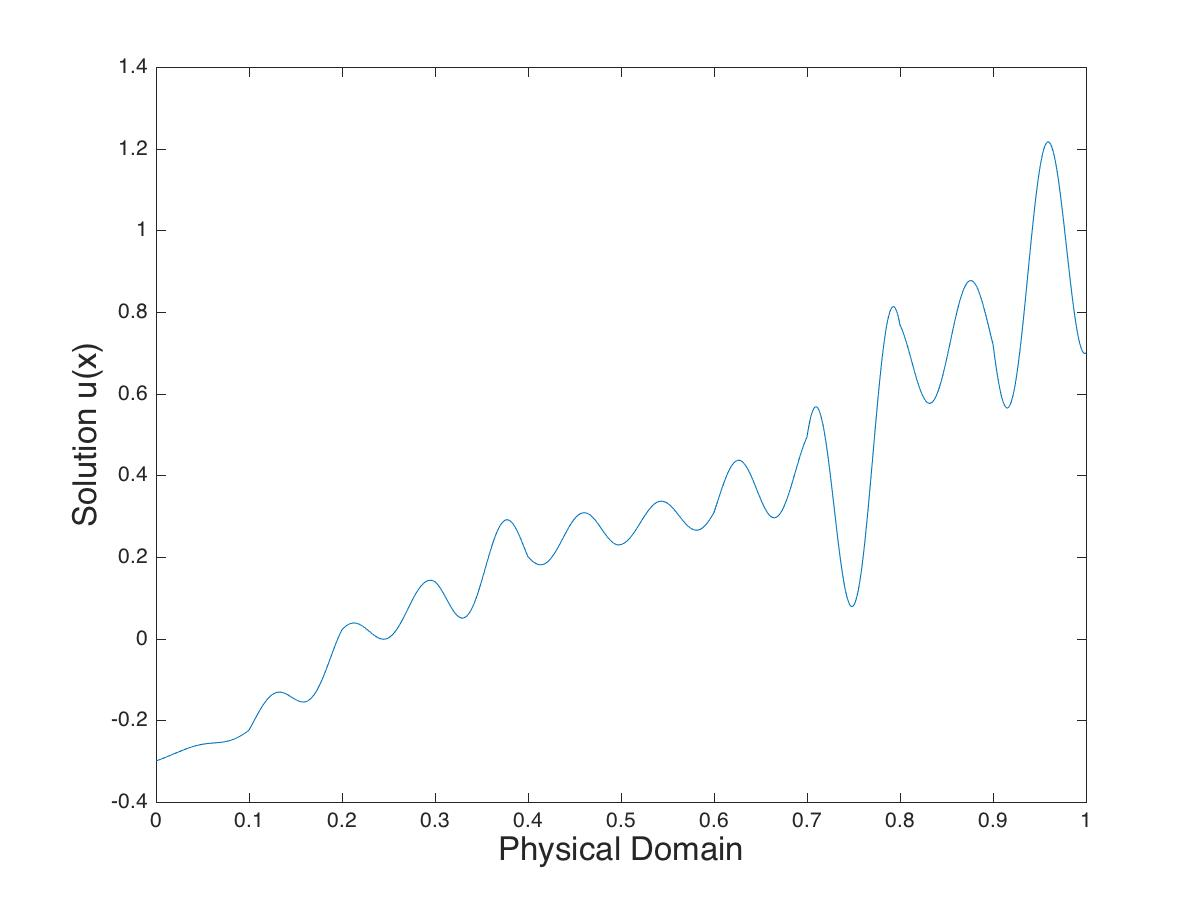
\includegraphics[width=0.75\linewidth]{AnalyticalSoln2.jpg}
\caption{Analytical solution.}
\end{center}
\end{figure}

\begin{table}[H]
\caption{Coefficients \(C_1\) and \(C_2\) over each domain of the problem.}
\centering
\begin{tabular}{c c r}
\hline\hline
Domain & \(C_1\) & \(C_2\)\\ [0.5ex]
\hline
\(0.0\leq x< 0.1\) & 1.9052  & -0.3000\\
\(0.1\leq x< 0.2\) & 1.9052  & -0.4133\\
\(0.2\leq x< 0.3\) & 1.9052  & -0.2269 \\
\(0.3\leq x< 0.4\) & 1.9052  & -0.3733\\
\(0.4\leq x< 0.5\) & 1.9052  & -0.0605\\
\(0.5\leq x< 0.6\) & 1.9052  &  0.0171\\
\(0.6\leq x< 0.7\) & 1.9052  & -0.1774\\
\(0.7\leq x< 0.8\) & 1.9052  & -1.5201\\
\(0.8\leq x< 0.9\) & 1.9052  & -0.0900\\
\(0.9\leq x< 1.0\) & 1.9052  & -0.9012\\
\hline
\end{tabular}
\label{table:orders}
\end{table}



\subsection{Finite Element Implementation}

The Galerkin FEM achieves the best approximation property by approximating the true solution \(u(x)\) as \(u^N(x)\), where both \(u^N(x)\) and the test function \(\psi\) are expanded in the same set of \(N\) basis functions \(\phi\):

\begin{equation}
\label{eq:approx}
\begin{aligned}
u\approx u^N=\sum_{j=1}^{N}a_j\phi_j\\
\psi=\sum_{i=1}^{N}b_i\phi_i\\
\end{aligned}
\end{equation}

Galerkin's method is stated as:

\begin{equation}
r^N\cdot u^N=0
\end{equation}

where \(r^N\) is the residual. Hence, to formulate the weak form to Eq. \eqref{eq:Problem}, multiply Eq. \eqref{eq:Problem} through by \(\psi\) and integrate over all space, \(d\Omega\).

\begin{equation}
\int_{\Omega}^{}\frac{d}{dx}\left(E(x)\frac{du}{dx}\right)\psi d\Omega-\int_{\Omega}^{}xk^3\cos{(\gamma x)}\psi d\Omega=0
\end{equation}

Applying integration by parts to the first term:

\begin{equation}
-\int_{\Omega}^{}E(x)\frac{du}{dx}\frac{d\psi}{dx}d\Omega+\int_{\partial\Omega}^{}E(x)\frac{du}{dx}\psi d(\partial\Omega)-\int_{\Omega}^{}xk^3\cos{(\gamma x)}\psi d\Omega=0
\end{equation}

where \(\partial\Omega\) refers to one dimension lower than \(\Omega\), which for this case refers to evaluation at the endpoints of the domain. Hence, for this particular 1-D problem, the above reduces to:

\begin{equation}
\begin{aligned}
-\int_{0}^{L}E(x)\frac{du}{dx}\frac{d\psi}{dx}dx+ E(x)\frac{du}{dx}\psi\biggr\vert_{0}^{L}-\int_{0}^{L}xk^3\cos{(\gamma x)}\psi dx=0\\
\int_{0}^{L}E(x)\frac{du}{dx}\frac{d\psi}{dx}dx=-\int_{0}^{L}xk^3\cos{(\gamma x)}\psi dx+E(x)\frac{du}{dx}\psi\biggr\vert_{0}^{L}\\
\end{aligned}
\end{equation}

Inserting the approximation described in Eq. \eqref{eq:approx}:

\begin{equation}
\begin{aligned}
\int_{0}^{L}E(x)\frac{d\left(\sum_{j=1}^{N}a_j\phi_j\right)}{dx}\frac{d\left(\sum_{i=1}^{N}b_i\phi_i\right)}{dx}dx=-\int_{0}^{L}xk^3\cos{(\gamma x)}\sum_{i=1}^{N}b_i\phi_idx+E(x)\frac{du}{dx}\sum_{i=1}^{N}b_i\phi_i\biggr\vert_{0}^{L}\\
\end{aligned}
\end{equation}

Recognizing that \(b_i\) appears in each term, the sum of the remaining terms must also equal zero (i.e. basically cancel \(b_i\) from each term).

\begin{equation}
\begin{aligned}
\int_{0}^{L}E(x)\frac{d\left(\sum_{j=1}^{N}a_j\phi_j\right)}{dx}\frac{d\phi_i}{dx}dx=-\int_{0}^{L}xk^3\cos{(\gamma x)}\phi_idx+E(x)\frac{du}{dx}\phi_i\biggr\vert_{0}^{L}\\
\end{aligned}
\end{equation}

This equation can be satisfied for each choice of \(j\), and hence can be reduced to:

\begin{equation}
\begin{aligned}
\int_{0}^{L}E(x)\frac{d\left(a_j\phi_j\right)}{dx}\frac{d\phi_i}{dx}dx=-\int_{0}^{L}xk^3\cos{(\gamma x)}\phi_idx+E(x)\frac{du}{dx}\phi_i\biggr\vert_{0}^{L}\\
\end{aligned}
\end{equation}

This produces a system of matrix equations of the form:

\begin{equation}
\label{eq:MatrixEqn}
\textbf{K}\vv{a}=\vv{F}
\end{equation}

where:

\begin{equation}
\begin{aligned}
\label{eq:SystemEquations}
K_{ij}=\int_{0}^{L}E(x)\frac{d\phi_i}{dx}\frac{d\phi_j}{dx}dx\\
a_j=a_j\\
F_i=-\int_{0}^{L}xk^3\cos{(\gamma x)}\phi_idx+E(x)\frac{du}{dx}\phi_i\biggr\vert_{0}^{L}\\
\end{aligned}
\end{equation}

where the second term in \(F_i\) is only applied at nodes that have Neumann boundary conditions (since \(\psi\) satisfies the homogeneous form of the essential boundary conditions). The above equation governs the entire domain. \(\textbf{K}\) is an \(n \times n\) matrix, where \(n\) is the number of global nodes. The solution is contained within \(\vv{a}\). This matrix system is solved in this assignment by simple Gaussian elimination, such that \(\vv{a}=\textbf{K}^{-1}\vv{F}\).

Quadrature is used to perform the numerical integration because it is much faster, and more general, than symbolic integration of the terms appearing in Eq. \eqref{eq:SystemEquations}. In order for these equations to be useful with Gaussian quadrature, they must be transformed to the master element which exists over \(-1\leq\xi\leq1\):

\begin{equation}
\label{eq:GoverningEqnsIsoparametric}
\begin{aligned}
K_{ij}=\int_{0}^{L}E(x)\frac{d\phi_i}{dx}\frac{d\phi_j}{dx}dx\rightarrow\int_{-1}^{1}E(x(\xi))\frac{d\phi_i}{dx}\frac{d\phi_j}{dx}dx\left(\frac{dx}{d\xi}\frac{dx}{d\xi}\frac{d\xi}{dx}\right)\rightarrow\int_{-1}^{1}E(x(\xi))\frac{d\phi_i}{d\xi}\frac{d\phi_j}{d\xi}dx\left(\frac{d\xi}{dx}\right)\\
a_j=a_j\\
F_i=-\int_{0}^{L}xk^3\cos{(\gamma x)}\phi_idx\rightarrow-\int_{-1}^{1}x(\xi)k^3\cos{(\gamma x(\xi))}\phi_i\frac{dx}{d\xi}d\xi\\
\end{aligned}
\end{equation} 

where the second term in \(F_i\) has been dropped because there are no Neumann boundary conditions in this assignment. For linear elements, the shape functions have the following form and derivative over the master element:

\begin{equation}
\begin{aligned}
\phi_1(\xi)=\frac{1-\xi}{2},\quad\frac{d\phi_1(\xi)}{d\xi}=-1/2\\
\phi_2(\xi)=\frac{1+\xi}{2}, \quad\frac{d\phi_2(\xi)}{d\xi}=+1/2\\
\end{aligned}
\end{equation}

The transformation from the physical domain (\(x\)) to the parent domain (\(\xi\)) is done with an isoparametric mapping:

\begin{equation}
\label{eq:Mapping}
x(\xi)=\sum_{i=1}^{N} X_i\phi_i(\xi)
\end{equation}

where \(X_i\) are the coordinates in each element. This mapping is performed for each element individually. The Jacobian \(dx/d\xi\) is obtain from Eq. \eqref{eq:Mapping} by differentiation:

\begin{equation}
\frac{dx(\xi)}{d\xi}=\sum_{i=1}^{N} X_i\frac{d\phi_i(\xi)}{d\xi}
\end{equation}

With all these transformations from the physical domain to the isoparametric domain, Gaussian quadrature can be used. A 5-point quadrature rule is used (given in the problem statement). For the five-point quadrature rule, the weights \(w\) and sampling points \(x\) are:

\begin{equation}
\begin{aligned}
w=\left\lbrack\frac{322-13\sqrt{70}}{900}, \frac{322+13\sqrt{70}}{900}, \frac{128}{225}, \frac{322+13\sqrt{70}}{900}, \frac{322-13\sqrt{70}}{900}\right\rbrack\\
x=\left\lbrack-\frac{1}{3}\sqrt{5+2\sqrt{10/7}}, -\frac{1}{3}\sqrt{5-2\sqrt{10/7}}, 0, \frac{1}{3}\sqrt{5-2\sqrt{10/7}}, \frac{1}{3}\sqrt{5+2\sqrt{10/7}}\right\rbrack\\
\end{aligned}
\end{equation} 

Transformation to the isoparametric domain therefore easily allows construction of the local stiffness matrix and local force matrix. The actual numerical algorithm computes the elemental \(k(i,j)\) and \(b(i)\) by looping over \(i, j\), and the quadrature points. Because each calculation is computed over a single element, a connectivity matrix is used to populate the global stiffness matrix and the global forcing vector with the elemental matrices and vectors. See the Appendix for the full code used in this assignment. After the global matrix and vector are formed, the global matrix has a banded-diagonal structure. However, this approach is only needed for direct methods such as Gaussian elimination. Because a PCG method is used here, there is no need to assemble the global \(\textbf{K}\). This will be explained in more detail in \ref{sec:PCG}.

In order to apply the boundary conditions within the numerical context of the finite element method, the matrix equation in Eq. \eqref{eq:MatrixEqn} must be rewritten to reflect that some of the nodal values are actually already specified through the Dirichlet boundary conditions. 

\begin{equation}
\label{eq:condensation}
\begin{bmatrix}
	K_{kk} & K_{ku}\\
	K_{uk} & K_{uu}\\
\end{bmatrix}
\begin{bmatrix}
	x_k\\
	x_u\\
\end{bmatrix}
=
\begin{bmatrix}
	F_k\\
	F_u\\
\end{bmatrix}
\end{equation}

where \(k\) indicates a known quantity (specified through a boundary condition) and \(u\) indicates an unknown quantity.   Explicitly expanding this equation gives:

\begin{equation}
\begin{aligned}
K_{kk}x_k+K_{ku}x_u=F_k\\
K_{uk}x_k+K_{uu}x_u=F_u\\
\end{aligned}
\end{equation}

Solving this matrix system is sometimes referred to as ``static condensation,'' since the original matrix system in Eq. \eqref{eq:MatrixEqn} must be separated into its components. The nodes at which Dirichlet conditions are specified are ``known,'' while all other nodes, including Neumann condition nodes, are ``unknown,'' since it is the value of \(u\) that we are looking to find at each node. The second of these equations is the one that is solved in this assignment, since there are no natural boundary conditions. So, while the global \textbf{K} matrix is not formed, in principle the Dirichlet boundary conditions are stilled applied in this manner, by removing certain rows and columns of \textbf{K} and \(\vv{F}\) from the PCG solve.

Once the solution is obtained by the PCG method, the solution is transformed back to the physical domain (from the isoparametric domain) by solving a linear matrix system to determine the coefficients on the basis functions over each element (in the physical domain). For example, for a quadratic shape function, over one element with coordinates \(x_1, x_2,\) and \(x_3\), with solution values \(a_1, a_2,\) and \(a_3\), the following linear system solves for the coordinates on the shape function in the physical domain, in that element:

\begin{equation}
\label{eq:LinearSolve}
\begin{bmatrix}
1 & x_1 & x_1^2\\
1 & x_2 & x_2^2\\
1 & x_3 & x_3^2\\
\end{bmatrix}
\begin{bmatrix} A\\ B\\ C
\end{bmatrix}
=
\begin{bmatrix} a_1 \\ a_2 \\ a_3
\end{bmatrix}
\end{equation}

Each element is looped over to obtain the coefficients on the shape functions in the physical domain. This then transforms the solution back to the physical domain, and completes the FE solution.

\subsection{Error Estimates and Convergence Criteria}

The accuracy of the FE solution is estimated using the energy norm \(e^N\), defined as:

\begin{equation}
e^N=\frac{\|u-u^N\|}{\|u\|}
\end{equation}

where:

\begin{equation}
\|u\|=\sqrt{\int_{\Omega}^{}\frac{du}{dx}E\frac{du}{dx}}
\end{equation}

\begin{equation}
\|u-u^N\|=\sqrt{\int_{\Omega}^{}\frac{d(u-u^N)}{dx}E\frac{d(u-u^N)}{dx}}=\sqrt{\int_{\Omega}^{}\left(\frac{du}{dx}-\frac{du^N}{dx}\right)E\left(\frac{du}{dx}-\frac{du^N}{dx}\right)}
\end{equation}

The derivatives of the FE solution are determined according to:

\begin{equation}
\frac{du^N}{dx}=\frac{d}{dx}\sum_{j=1}^{N}a_j\phi_j(x)=\sum_{j=1}^{N}a_j\frac{d\phi_j(x)}{dx}=\sum_{j=1}^{N}a_j\frac{d\phi_j(x)}{d\xi}\frac{d\xi}{dx}
\end{equation}

while the derivative of the analytical solution is obtained from Eq. \eqref{eq:Problem2}. 

\subsection{The Preconditioned Conjugate Gradient Method}

The Preconditioned Conjugate Gradient (PCG) method is used to perform the numerical solution of the linear algebra system. This method is an iterative method, and computes the solution \(\vv{a}\) at each iteration by adding an update \(\vv{z}\) to the previous iterate, scaled by a constant \(\lambda\):

\begin{equation}
\label{eq:PCGUpdate}
\vv{a}^{i+1}=\vv{a}^i+\lambda^i\vv{z}^i
\end{equation}

where \(i\) denotes the iteration number. This requires an initial guess for \(\vv{a}^1\) (indexing starts at 1). Because the nodes at which Dirichlet boundary conditions apply have already been removed, this initial guess is set, for simplicity, to values of 1 at all nodes. Physics-based preconditioning is a more sophisticated method that takes into account more realistic solutions to provide the initial guess for the solution, but this is not pursued here. Due to the similarity between the PCG method and the Method of Steepest Descent, for simplicity, the initial guess for \(\vv{z}^1\) is chosen to be the residual when evaluate with \(\vv{a}^1\). The residual \(\vv{r}\) is here defined to be:

\begin{equation}
\vv{r}^i=\vv{F}-\textbf{K}\vv{a}^i
\end{equation}

The quantity \(\vv{z}^i\) is chosen to be K-conjugate to the previous iterate \(\vv{z}^{i-1}\). This weighted inner product searches, in the next iterate, in the conjugate gradient direction of the previous iterate, while taking into account the structure of the governing equation. In other words, it is required that:

\begin{equation}
\vv{z}^{i,T}\textbf{K}\vv{z}^{i-1}=0
\end{equation}

This then gives the following form for \(\theta\):

\begin{equation}
\theta^i=-\frac{\vv{r}^{T,i}\textbf{K}\vv{z}^{i-1}}{\vv{z}^{T,i-1}\textbf{K}\vv{z}^{i-1}}
\end{equation}

where \(\theta\) is used in the update of \(\vv{z}\) as:

\begin{equation}
\vv{z}^i=\vv{r}^i+\theta^i\vv{z}^{i-1}
\end{equation}

By solving for \(\lambda^i\) in Eq. \eqref{eq:PCGUpdate} and substituting this into the potential function that minimizes the potential energy of the FE solution, the following optimal form for \(\lambda^i\) is found:

\begin{equation}
\lambda^i=\frac{\vv{z}^{T,i}\vv{r}^i}{\vv{z}^{T,i}\textbf{K}\vv{z}^i}
\end{equation}

The point at which the iterations are stopped is based on the energy norm discussed in the previous section. The error tolerance for the PCG method is set to 0.000001, and so the iterations are halted once:

\begin{equation}
\left(\vv{a}^{T,i+1}-\vv{a}^{T,i}\right)\textbf{K}\left(\vv{a}^{i+1}-\vv{a}^i\right)<0.000001
\end{equation}

The PCG method has convergence behavior dictated by:

\begin{equation}
\|\vv{a}-\vv{a}^{i}\|_K\leq\left(\frac{\sqrt{C(\textbf{K})}-1}{\sqrt{C(\textbf{K})}+1}\right)^i\|\vv{a}-\vv{a}^1\|_K
\end{equation}

In other words, the convergence speed is governed by the condition number. The identity matrix has the lowest possible condition number of 1, but real physical problems tend to have much larger condition numbers. The higher the condition number, then the slower the rate of convergence. Preconditioning can be used to transform the linear system \(\textbf{K}\vv{a}=\vv{R}\) to a different domain in which the condition number is higher. The preconditioning matrix \textbf{T} is used to introduce this change of variables:

\begin{equation}
\label{eq:Transformation}
\textbf{K}\vv{a}=\vv{R}\quad\rightarrow\hat{\textbf{K}}\hat{\vv{a}}=\hat{\vv{R}}
\end{equation}

where

\begin{equation}
\label{eq:TransformationSpecs}
\begin{aligned}
\hat{\vv{a}}=\textbf{T}^{-1}\vv{a}\\
\hat{\textbf{K}}=\textbf{T}^{T}\textbf{K}\textbf{T}\\
\hat{\vv{R}}=\textbf{T}^T\vv{R}\\
\end{aligned}
\end{equation}

Then, it is the condition number of \(\hat{\textbf{K}}\) that controls the convergence. The best possible preconditioner is to set \(\textbf{T}=\textbf{L}^{-T}\), where \(\textbf{L}\textbf{L}^T=\textbf{K}\) and \textbf{L} is a lower-triangular matrix. With this preconditioner, Eq. \eqref{eq:Transformation} becomes:

\begin{equation}
\label{eq:Transformation2}
\underbrace{\textbf{L}^{-1}\textbf{L}}_\text{\textbf{I}}\underbrace{\textbf{L}^T\textbf{L}^{-T}}_\text{\textbf{I}}\hat{\vv{a}}=\hat{\vv{R}}
\end{equation}

which then gives \(\textbf{I}\hat{\vv{a}}=\hat{\vv{R}}\), which is an incredibly easy system to solve numerically, since then \(\hat{\vv{a}}=\hat{\vv{R}}\). However, the cost to form \(\textbf{L}\) is of order \(N^3\), and hence defeats the purpose of using the PCG method, since standard Gaussian elimination also scales as approximately \(N^3\). Hence, a simpler preconditioner is selected here. For this assignment, a diagonal preconditioner is used:

\begin{equation}
T_{ij}=\frac{1}{\sqrt{K_{ij}}}\delta_{ij}
\end{equation}

where \(\delta_{ij}\) is the Kronecker delta. With this preconditioner, the transformations described in Eq. \eqref{eq:TransformationSpecs} are made. Then, the PCG method described earlier is performed on this preconditioned system. Once reaching an acceptable error tolerance, the result is transformed back to the actual problem domain to give the final result.

\section{Solution Results and Discussion}



\section{Appendix}

This section contains the code used for this modeling. The main program is \texttt{FEProgram.m}, and functions perform specialized tasks for a high degree of modularity.

\subsection{\texttt{FEProgram.m}}
This is the main code used for the problem solving.
\lstinputlisting[language=Matlab]{FEProgram.m}

\subsection{\texttt{BCnodes.m}}
This function applies boundary conditions.
\lstinputlisting[language=Matlab]{BCnodes.m}

\subsection{\texttt{condensation.m}}
This function separates out the matrix equation as in Eq. \eqref{eq:condensation}.
\lstinputlisting[language=Matlab]{condensation.m}

\subsection{\texttt{ElementInterpolation.m}}
This function interpolates the block-structure of \(E\) into an elemental basis (\(E\) as a function of the element number).
\lstinputlisting[language=Matlab]{ElementInterpolation.m}

\subsection{\texttt{mesh.m}}
This function performs the meshing.
\lstinputlisting[language=Matlab]{mesh.m}

\subsection{\texttt{PCG.m}}
This function performs the Preconditioned Conjugate Gradient solve of the matrix system.
\lstinputlisting[language=Matlab]{PCG.m}

\subsection{\texttt{permutation.m}}
This function determines the permutation matrix for use with the connectivity matrix.
\lstinputlisting[language=Matlab]{permutation.m}

\subsection{\texttt{PhysicalInterpolation.m}}
This function interpolates a block-structure \(E\) into the physical domain (\(E\) as a function of position).
\lstinputlisting[language=Matlab]{PhysicalInterpolation.m}

\subsection{\texttt{postprocess.m}}
This function postprocesses the FE solution and transforms it back to the physical domain using a linear system solve as described in Eq. \eqref{eq:LinearSolve}.
\lstinputlisting[language=Matlab]{postprocess.m}

\subsection{\texttt{quadrature.m}}
This function selects the quadrature rule.
\lstinputlisting[language=Matlab]{quadrature.m}

\subsection{\texttt{RHSFunction.m}}
This function repeatedly evaluates \circled{A} for determination of the analytical solution.
\lstinputlisting[language=Matlab]{RHSFunction.m}

\subsection{\texttt{shapefunctions.m}}
This function contains the library of shape functions.
\lstinputlisting[language=Matlab]{shapefunctions.m}




\end{document}